% Copyright 2015--2017  Ed Bueler

\documentclass[10pt,hyperref]{beamer}

\mode<presentation>
{
  \usetheme{Madrid}

  \usecolortheme{beaver}

  \setbeamercovered{transparent}
  
  \setbeamerfont{frametitle}{size=\large}
}

\setbeamercolor*{block title}{bg=red!10}
\setbeamercolor*{block body}{bg=red!5}

\usepackage[english]{babel}
\usepackage[latin1]{inputenc}
\usepackage{times}
\usepackage[T1]{fontenc}
% Or whatever. Note that the encoding and the font should match. If T1
% does not look nice, try deleting the line with the fontenc.

\usepackage{empheq}
\usepackage{animate}
\usepackage{xspace}
\usepackage{fancyvrb}
\usepackage{hyperref}



\title{Classical iterative methods for linear systems}

\author{Ed Bueler}

\institute[MATH 615 NADEs]{MATH 615 Numerical Analysis of Differential Equations}

\date[Spring 2017]{27 February--1 March, 2017}



% If you wish to uncover everything in a step-wise fashion, uncomment
% the following command: 
%\beamerdefaultoverlayspecification{<+->}

\newcommand{\bb}{\mathbf{b}}
\newcommand{\bc}{\mathbf{c}}
\newcommand{\br}{\mathbf{r}}
\newcommand{\bx}{\mathbf{x}}
\newcommand{\by}{\mathbf{y}}
\newcommand{\bv}{\mathbf{v}}
\newcommand{\bu}{\mathbf{u}}
\newcommand{\bw}{\mathbf{w}}

\newcommand{\CC}{\mathbb{C}}
\newcommand{\RR}{\mathbb{R}}

\newcommand{\ddt}[1]{\ensuremath{\frac{\partial #1}{\partial t}}}
\newcommand{\ddx}[1]{\ensuremath{\frac{\partial #1}{\partial x}}}
\renewcommand{\t}[1]{\texttt{#1}}
\newcommand{\Matlab}{\textsc{Matlab}\xspace}
\newcommand{\Octave}{\textsc{Octave}\xspace}
%\newcommand{\MO}{\Matlab/\Octave}
\newcommand{\MO}{\Matlab}
\newcommand{\eps}{\epsilon}

\newcommand{\MS}{\alert{MAKE SURE}\xspace}

\newcommand{\exer}[2]{\medskip\noindent \textbf{#1.}\quad #2}

\newcommand{\mfile}[1]{
\VerbatimInput[frame=single,label=\fbox{\scriptsize \textsl{\,#1\,}},fontfamily=courier,fontsize=\scriptsize]{#1}
}

\newcommand{\mfiletiny}[1]{
\VerbatimInput[frame=single,label=\fbox{\scriptsize \textsl{\,#1\,}},fontfamily=courier,fontsize=\tiny]{#1}
}


\AtBeginSection[]
{
  \begin{frame}<beamer>
    \frametitle{Outline}
    \tableofcontents[currentsection,hideallsubsections]
  \end{frame}
}

\begin{document}

\begin{frame}
  \maketitle
\end{frame}


\begin{frame}{example linear systems}

\begin{itemize}
\item suppose we want to solve the linear system
\begin{equation}
A \bx = \bb \label{introsystem}
\end{equation}
where $A\in \RR^{m\times m}$ and $\bb\in \RR^m$, to find $\bx\in \RR^m$.
\item  throughout these notes we use just two examples:
  \begin{itemize}
  \item[LS1] 
\begin{equation*}
\begin{bmatrix} 2 & 1 & 0 \\
                0 & 2 & 1 \\
                1 & 0 & 3 \end{bmatrix}
\begin{bmatrix} x_1 \\ x_2 \\ x_3 \end{bmatrix}
=
\begin{bmatrix} 2 \\ 1 \\ 4 \end{bmatrix}
\end{equation*}
  \item[LS2]
\begin{equation*}
\begin{bmatrix} 1 & 2 & 3 & 0 \\
                2 & 1 &-2 &-3 \\
               -1 & 1 & 1 & 0 \\
                0 & 1 & 1 &-1 \end{bmatrix}
\begin{bmatrix} x_1 \\ x_2 \\ x_3 \\ x_4 \end{bmatrix}
=
\begin{bmatrix} 7 \\ 1 \\ 1 \\ 3 \end{bmatrix}
\end{equation*}
  \end{itemize}
\item on \textbf{P17} (Assignment \#5) you will check that these are well-conditioned linear systems
\item it is trivial to find solutions of LS1, LS2 using a ``$\bx = A\backslash \bb$'' black box, but these examples stand-in for the large linear systems we get from applying FD schemes to ODE and PDE problems
\end{itemize}
\end{frame}


\begin{frame}{residual}

\begin{itemize}
\item the \emph{residual} of a vector $\bv$ in linear system \eqref{introsystem} is the vector
\begin{equation}
\br(\bv) = \bb - A \bv \label{residualdefn}
\end{equation}
\item making the residual zero is the same as solving the system:
      $$A \bx=\bb \, \iff \, \br(\bx)=0$$
\item evaluating $\br(\bv)$ needs a matrix-vector product and a vector subtraction
  \begin{itemize}
  \item[$\circ$] requires $O(m^2)$ operations at worst
  \item[$\circ$] by comparison, applying Gauss elimination to solve linear system \eqref{introsystem} is an $O(m^3)$ operation in general
  \end{itemize}
\item FD schemes for DEs generate matrices $A$ for which the majority, often $99\%$ or more, of the entries are zero
  \begin{itemize}
  \item[$\circ$] a matrix with enough zeros to allow exploitation of that fact is called \emph{sparse}
  \item[$\circ$] evaluating the residual of a sparse matrix typically requires $O(m)$ operations
  \item[$\circ$] even if $A$ is sparse, $A^{-1}$ is generally \emph{dense}, i.e.~most entries are nonzero
  \end{itemize}
\end{itemize}
\end{frame}


\begin{frame}{Richardson iteration}

\begin{itemize}
\item \emph{iterative methods} for linear system \eqref{introsystem} attempt to solve it based only on operations like computing the residual, or applying $A$ to a vector
  \begin{itemize}
  \item[$\circ$] one wants the sequence of approximations, the iterates, to \emph{converge} to the solution $\bx = A^{-1} \bb$
  \item[$\circ$] Iterative methods always require an initial iterate $\bx_0$
  \end{itemize}
\item \emph{Richardson iteration} adds a multiple $\omega$ of the last residual at each step:
\begin{equation}
\bx_{k+1} = \bx_k + \omega (\bb - A \bx_k)  \label{richardson}
\end{equation}
\item for system LS1, using initial iterate $\bx_0=0$ and $\omega=1/5$, \eqref{richardson} gives:\small
\begin{align*}
\bx_0 &= \begin{bmatrix} 0 \\ 0 \\ 0 \end{bmatrix}, \,
\bx_1 = \begin{bmatrix} 0.4 \\ 0.2 \\ 0.8 \end{bmatrix}, \,
\bx_2 = \begin{bmatrix} 0.6 \\ 0.16 \\ 1.04 \end{bmatrix}, \,
\bx_3 = \begin{bmatrix} 0.728 \\ 0.088 \\ 1.096 \end{bmatrix}, \, \dots, \,
\bx_{10} = \begin{bmatrix} 0.998 \\ -0.017 \\ 1.01 \end{bmatrix},
\dots
\end{align*}
these iterates seem to be converging to $\bx = [1 \,\, 0 \,\, 1]^\top$, which is the solution to LS1
\end{itemize}
\end{frame}


\begin{frame}{recall: eigenvalues and vectors}

\begin{itemize}
\item a complex number $\lambda \in \CC$ is an \emph{eigenvalue} of a square matrix $B\in\RR^{m\times m}$ if there is a nonzero vector $\bv\in\CC^m$ so that $B \bv = \lambda \bv$
\item the set of all eigenvalues of $B$ is the \emph{spectrum} $\sigma(B)$ of $B$
\item the \emph{spectral radius} $\rho(B)$ is the maximum absolute value of an eigenvalue:
    $$\rho(B) = \max_{\lambda\in\sigma(B)}  |\lambda|$$
\item even if $B$ is real, $\lambda$ may be complex---the roots of a polynomial with real coefficients may be complex---\emph{and} if $\lambda$ is complex and $B$ is real then $\bv$ must be complex
\end{itemize}
\end{frame}


\begin{frame}{spectral properties and convergence of iterations}

\begin{itemize}
\item properties of a matrix $B$ described in terms of eigenvalues are generically called \emph{spectral properties}
\item some examples:
  \begin{itemize}
  \item[$\circ$] $\rho(B)$
  \item[$\circ$] $\|B\|_2 = \sqrt{\rho(B^\top B)}$
  \item[$\circ$] the 2-norm condition number $\kappa(B)=\|B\|_2 \|B^{-1}\|_2$
  \end{itemize}

\medskip
\item a general idea:
\begin{quote}
whether an iterative method for solving $A\bx = \bb$ converges, or not, depends on spectral properties of $A$, or on matrices built from $A$
\end{quote}

\medskip
\item the right-hand side $\bb$ and the initial iterate $\bx_0$ generally \emph{do not} determine whether an iteration converges
  \begin{itemize}
  \item[$\circ$] a good choice of $\bx_0$ \emph{can} speed up convergence
  \end{itemize}
\end{itemize}
\end{frame}


\begin{frame}{convergence of the Richardson iteration}

\begin{itemize}
\item rewrite the Richardson iteration \eqref{richardson} as
    $$\bx_{k+1} = (I - \omega A) \bx_k + \omega \bb$$
\item the lemma on the next slide shows that the Richardson iteration converges if and only if all the eigenvalues of the matrix $I-\omega A$ are inside the unit circle:
    $$\text{\eqref{richardson} converges if and only if } \rho(I-\omega A) < 1$$
  \begin{itemize}
  \item[$\circ$] $\rho(I-\omega A) < 1$ means $(I - \omega A) \bx_k$ is smaller in magnitude than $\bx_k$
  \item[$\circ$] \emph{if} $\|I-\omega A\| < 1$ \emph{then} \eqref{richardson} converges\footnote{recall $\rho(B) \le \|B\|$ in any induced matrix norm}
  \end{itemize}
\end{itemize}
\end{frame}


\begin{frame}{convergence lemma}

\begin{lemma}
   $$\by_{k+1} = M \by_k + \bc$$
converges to the solution of $\by = M \by + \bc$ for all initial $\by_0$ if and only if
   $$\rho(M) < 1.$$
\end{lemma}

\small
\begin{proof}
Solve the iteration by writing out a few cases:
\begin{align*}
   \by_2 &= M (M \by_0 + \bc) + \bc = M^2 \by_0 + (I + M) \bc, \\
   \by_3 &= M (M^2 \by_0 + (I + M) \bc) + \bc = M^3 \by_0 + (I + M + M^2) \bc, \\
   &\vdots
\end{align*}
By induction we get $\by_k = M^k \by_0 + p_k(M) \bc$ where $p_k(x) = 1 + x + x^2 + \dots + x^{k-1}$.  But $p_k(x) \to 1/(1-x)$ as $k\to\infty$ iff $x\in(-1,1)$.  Also, $\rho(M)<1$ iff $M^k \to 0$.  Thus $\by_k \to (I-M)^{-1} \bc$ iff $\rho(M) < 1$.
\end{proof}
\end{frame}


\begin{frame}[fragile]{convergence of the Richardson iteration 2}

\begin{itemize}
\item since the Richardson iteration converges iff $\rho(I - \omega A)<1$, we choose $\omega$ based on the principle that
    $$\omega A \text{ should be close to the identity } I$$
\vspace{-5mm}
  \begin{itemize}
  \item[$\circ$] often not possible!
  \end{itemize}

\medskip
\item in small cases we can graph $f(\omega) = \rho(I-\omega A)$:

\medskip
\begin{columns}
\begin{column}{0.5\textwidth}
\footnotesize
\begin{verbatim}
   omega = -1:.01:1;
   rho = zeros(size(omega));
   for j = 1:length(omega)
       M = eye(n) - omega(j) * A;
       rho(j) = max(abs(eig(M)));
   end
   plot(omega,rho)
\end{verbatim}

\smallskip
\begin{itemize}
\footnotesize
\item[for LS1:]  $\rho(I - \omega A)$ dips below $1$ for $0 < \omega \lesssim 0.6$
\item[for LS2:]  $\rho(I - \omega A) \ge 1$ always
\end{itemize}
\end{column}

\begin{column}{0.4\textwidth}
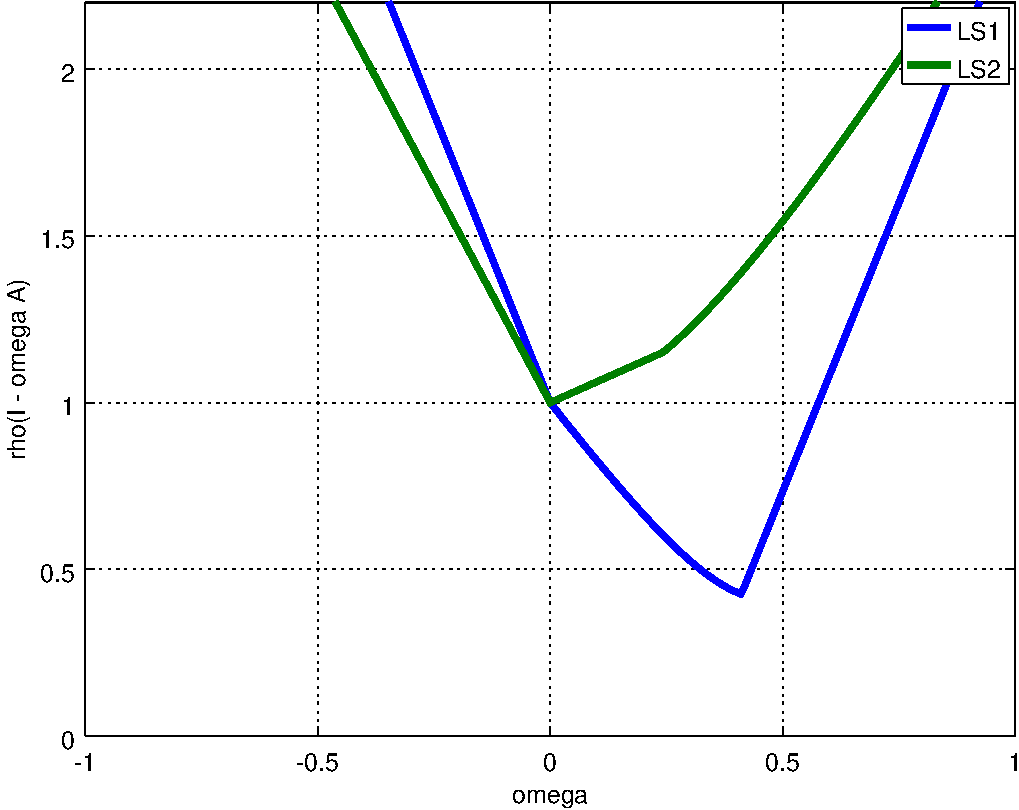
\includegraphics[width=2.0in,keepaspectratio=true]{richardspect}
\end{column}
\end{columns}

\medskip
\item  note $\rho(I-0A)=1$ \, \dots \, so no convergence when $\omega \approx 0$
\item  for LS1, figure suggests $\omega \approx 0.4$ gives fastest convergence
\end{itemize}
\end{frame}


\begin{frame}{matrix splitting}

\begin{itemize}
\item unlike Richardson, most classical iteration methods ``split'' the matrix $A$ before iterating
\item the best known, and simplest, iteration based on splitting is \emph{Jacobi iteration}, which extracts the diagonal of $A$ (and inverts it)
\item the splitting we consider is
    $$A = D - L - U \vspace{-3mm}$$
where
  \begin{itemize}
  \item[$\circ$] $D$ is the diagonal of $A$
  \item[$\circ$] $L$ is strictly lower triangular ($\ell_{ij} = 0$ if $i \le j$)
  \item[$\circ$] $U$ is strictly upper triangular ($u_{ij} = 0$ if $i \ge j$)
  \end{itemize}
\item you can split \emph{any} matrix this way
\item see section 4.2 of the textbook

\medskip
\item so that $D$ is an invertible matrix, for the remaining slides we assume

\centerline{\emph{all diagonal entries of $A$ are nonzero}: \quad  $a_{ii} \ne 0$}
\end{itemize}
\end{frame}


\begin{frame}{Jacobi iteration}

\begin{itemize}
\item the Jacobi iteration is
\begin{equation}
D \bx_{k+1} = \bb + (L + U) \bx_k  \label{jacobi}
\end{equation}
\item if it converges then $D\bx = \bb + (L+U)\bx$, which is the same as $A \bx = \bb$
\item we could also write it as \quad $\bx_{k+1} = D^{-1} \left(\bb + (L + U) \bx_k\right)$ \quad or as
\begin{equation}
x_i^{(k+1)} = \frac{1}{a_{ii}} \left(b_i - \sum_{j\ne i} a_{ij} x_j^{(k)}\right)  \label{jacobiA}
\end{equation}
where $x_j^{(k)}$ denotes the $j$th entry of the $k$th iterate $\bx_k$

\medskip
\item make sure you understand why \eqref{jacobi} and \eqref{jacobiA} are the same!
\end{itemize}
\end{frame}


\begin{frame}{Gauss-Seidel iteration}

\begin{itemize}
\item \emph{Gauss-Seidel iteration} extracts the non-strict lower-triangular part of $A$ (and inverts it)
\item again if $A = D - L - U$ then it is
\begin{equation}
(D - L) \bx_{k+1} = b + U \bx_k  \label{gaussseidel}
\end{equation}
\item we could also write it \quad ``\,$\bx_{k+1} = (D-L)^{-1} \left(b + U \bx_k\right)$\,'' \quad but that would miss the point!
\item instead we write it as \quad $D \bx_{k+1} = b + U \bx_k + L \bx_{k+1}$ \quad or equivalently:
\begin{equation}
x_i^{(k+1)} = \frac{1}{a_{ii}} \left(b_i - \sum_{j > i} a_{ij} x_j^{(k)} - \sum_{j < i} a_{ij} x_j^{(k+1)}\right)  \label{gaussseidelA}
\end{equation}
\item the lower-triangular entries of $A$ apply to \emph{those entries of $\bx_{k+1}$ which have already been computed}
\item form \eqref{gaussseidelA} is actually \emph{easier} to implement than Jacobi \eqref{jacobiA}  \quad (why?)
\end{itemize}
\end{frame}


\begin{frame}{convergence conditions for Jacobi and Gauss-Seidel}

\begin{itemize}
\item the convergence lemma says that
  \begin{itemize}
  \item[$\circ$] Jacobi iteration converges if and only if $\rho(D^{-1} (L+U)) < 1$
  \item[$\circ$] Gauss-Seidel iteration converges if and only if $\rho((D-L)^{-1} U) < 1$
  \end{itemize}
\item these conditions are hard to use in practice because computing a spectral radius can be just as hard as solving the original system
\end{itemize}
\end{frame}


\begin{frame}{diagonally-dominant matrices}

\begin{itemize}
\item \emph{definition}.  $A$ is \emph{strictly diagonally-dominant} if $|a_{ii}| > \sum_{j\ne i} |a_{ij}|$
  \begin{itemize}
  \item[$\circ$] LS1 is strictly diagonally-dominant
  \item[$\circ$] LS2 is not
  \end{itemize}

\item two relatively-famous theorems\footnote{section 11.2 of Golub and van Loan, \emph{Matrix Computations}, 4th edition 2013} are these:
  \begin{itemize}
  \item[$\circ$] if $A$ is strictly diagonally-dominant then both the Jacobi and Gauss-Seidel iterations converge 
  \item[$\circ$] if $A$ is symmetric positive definite then Gauss-Seidel iteration converges
  \end{itemize}
\item unlike the ``$\rho(\dots) < 1$'' conditions on the last slide:
  \begin{itemize}
  \item[$\circ$] it is easy to check diagonal-dominance, and it is a common property of the matrices coming from FD schemes on ODEs and PDEs
  \item[$\circ$] these are only \emph{sufficient} conditions, e.g.~there are nonsymmetric $A$, which are \emph{not} diagonally-dominant, but for which the iterations converge
  \end{itemize}

\medskip
\item see problems \textbf{P19} and \textbf{P20}
\end{itemize}
\end{frame}


\begin{frame}{past}

\begin{itemize}
\item the Jacobi and Gauss-Seidel iterations are from the 19th century
  \begin{itemize}
  \item[$\circ$] Richardson iteration first appears in a 1910 publication
  \end{itemize}
\item the early history of numerical partial differential equations, e.g.~in the 1920 to 1970 period, heavily used these classical iterations
  \begin{itemize}
  \item[$\circ$] a generalization of Gauss-Seidel iteration called \emph{successive over-relaxation}, was a particular favorite around 1970;  see section 4.2 of the textbook
  \end{itemize}
\item none of these iterations work on system LS2
\end{itemize}
\end{frame}


\begin{frame}{recent past and future}

\begin{itemize}
\item there are better iterative ideas, and they flourished starting in the 1980-90s \dots and far into the future
  \begin{itemize}
  \item[$\circ$] among the best known are CG = \emph{conjugate gradients} (actually from 1950-60s) and GMRES = \emph{generalized minimum residuals} (from a 1986 paper by Saad and Schultz)
  \item[$\circ$] GMRES works (i.e.~converges at some rate) on LS2
  \item[$\circ$] \emph{but} there can be no ``good iteration'' with a universally-fast convergence rate\footnote{remarkably, there is a 1992 theorem by Nachtigal, Reddy, and Trefethen that says this}
\end{itemize}

\medskip 
\item iteration to solve linear systems is the future:
  \begin{itemize}
  \item[$\circ$] it is obligatory on sufficiently-big systems
  \item[$\circ$] it works better in parallel than direct methods like Gauss elimination
  \item[$\circ$] it can exploit partial knowledge of the underlying model
  \end{itemize}
\end{itemize}
\end{frame}


\begin{frame}{biographies}

\begin{itemize}
\small
\item Gauss (1777--1855) did big stuff, not just the little Gauss-Seidel thing:

    \centerline{\href{https://en.wikipedia.org/wiki/Carl_Friedrich_Gauss}{\texttt{en.wikipedia.org/wiki/Carl\_Friedrich\_Gauss}}}

\medskip
\item Jacobi (1804--1851) also has his name on the ``Jacobian'', the matrix of derivatives appearing in Newton's method for systems of equations:

    \centerline{\href{https://en.wikipedia.org/wiki/Carl_Gustav_Jacob_Jacobi}{\texttt{en.wikipedia.org/wiki/Carl\_Gustav\_Jacob\_Jacobi}}}

\medskip
\item Seidel (1821--1896) is relatively little known:

    \centerline{\href{https://en.wikipedia.org/wiki/Philipp_Ludwig_von_Seidel}{\texttt{en.wikipedia.org/wiki/Philipp\_Ludwig\_von\_Seidel}}}

\medskip
\item Richardson (1881--1953) is the most interesting.  He invented numerical weather forecasting, doing it by-hand for fun during WWI.  Later, as a pacifist and quaker, he quit the subject entirely when he found his meteorological work was of most value to chemical weapons engineers and the British Air Force:

    \centerline{\href{https://en.wikipedia.org/wiki/Lewis_Fry_Richardson}{\texttt{en.wikipedia.org/wiki/Lewis\_Fry\_Richardson}}}
\end{itemize}
\end{frame}

\end{document}

